
%\begin{figure}[t]
%\centering
%\includegraphics[scale=1,clip]{figure/n2n.eps}\vspace*{-3ex}
% \caption{Merging technique}\vspace*{-3.5ex}
% \label{fig:n2n}
%\end{figure}

\section{Discussion and Future Work}
\label{sec:discuss}

We next discuss issues in our approach and describe how we address
these issues in our future work.

\textbf{Detecting more behavioral difference of mapped API elements.} Although our approach detected many behavioral differences, it may fail to reveal all behaviors. To detect more behavioral differences, some directions seem to be promising: (1) we can rely on side effects or  mock objects to test methods without return values; (2) to test API methods that return random values, we can check the distribution of their returned values; (3) other tools such as CUTE~\cite{koushik:cute} and JPF~\cite{visser2003mcp} may help generate more test cases to reveal more behaviors. We plan to explore these directions in future work. In addition, our approach does not cover some types of API elements (\emph{e.g.}, abstract classes and protected elements). To test these elements, we plan to extend our wrappers in future work (\emph{e.g.}, generating a concrete wrapper class for each abstract class). In our project website, we released all synthesized and translated wrappers, so that other researchers can also employ other static/dynamic techniques to detect more behavioral differences.

\textbf{Testing translation of other programming languages.} Some programming languages may have much more different code structures than Java and C\# do, and existing translation tools between these programming languages may fail to translate some different code structures. Daniel \emph{et al.}~\cite{daniel2007automated} propose an approach that tests refactoring engines by comparing their refactored results given the same generated abstract syntax trees. In future work, we plan to adapt their approach to test translation tools by comparing their translation results given the same code structures as inputs. As pointed out by Waters~\cite{waters1988program}, when a source language is fundamentally different from its target language, programmers may even have to abstract a source program and to re-implement its target program from scratch. Still, API differences are important for programmers to avoid related defects when they re-implement a target program. Canfora \emph{et al.}~\cite{CanforaFFT08} propose an approach that can wrap functionalities of legacy system as services. To detect such differences, we plan to adapt their wrappers to test mapped API elements between two fundamentally different languages in future work.

\textbf{Improving translation tools and detecting related defects.} Our evaluation reveals where existing tools fail to fix behavioral differences between mapped API elements. To improve existing translation tools, we plan to mine better mapping relations and to propose corresponding translation techniques for fixing these differences. In addition, found behavioral differences are potential to introduce defects in translated client code. In future work, we plan to conduct empirical studies to investigate whether found behavior differences really introduced defects in translated code, and to propose corresponding detection techniques if such defects are found.

%\textbf{Testing API mapping of single language.} We find that many existing approaches translate applications within single languages. For example, twinning~\cite{nita2010using} translates applications based on mapping relations of API invocations from different API libraries, and CatchUp!~\cite{henkel2005catchup} translates applications based on mapping relations of API invocations from different versions. In future work, we plan to adapt our approach to test mapping relations of API invocations within single languages. 